%% Encoding: ISO8859-1 %%

% In all of the following, please set NAME as your name in \citeNAME, 
% \includegraphics[...]{NAME/images/...}, \bibliographystyleNAME, and
% \bibliographyNAME{NAME/Literature}


\Paper{LOGSPACE, RandomWalks on Graphs and Universal Traversal Sequences}{Patrick Niklaus} % Please specify title of your work and your full name here
\newtheorem{thm}{Theorem}

In this paper I will present the collected findings of Aleliunas et. al.
\citeNiklaus{aleliunas1979random} on the space complexity of deciding
whether there exsists a path between two nodes $a$, $b$ in graphs.

Interestingly the complexity of this decision problem is different for
directed and undirected graphs. These differences can be exploited to
characterize the two space-bounded complexity classes $L$ and $NL$.

In the case of an undirected graph, we can employ an algorithm called
\emph{random walk} which does just that. Unlike common path finding
algorithms like the famous Dijekstra algorithm, this algorithm only
needs a logarithmic amount of storage to compute, and is inherently
simplistic in its decription: Instead of chosing the next neighbour node
to explore based on certain criteria, we just pick one at random and
check if we reached our destination. It is not intuetively clear that
this algorithm can decide whether there is a path between $a$ and $b$
correctly. Infact it can only do so with a certain probability, it is an
\emph{randomized} algorithm. However, by chosing a sufficent number of
steps we can make sure it decides correctly with a probability higher
than $\frac{1}{2}$, which we can still increase by just running the
algorithm multiple times.

Furthermore this is deeply related to finding ``routing directions'',
that visit all nodes in a graph and work in all graphs with a certain
size, so called \emph{universal traversal sequences}. We will show that
for every graph that is $d-connected$, there exists such a sequences and
its length is only polynominal in the number of nodes.

\paragraph{Further Research}\label{further-research}

A lot of research has be done by Aldous et. al on providing tighter
lower bounds for the minium number of steps it takes to visit all nodes
in graph, both for special graphs e.g.~b-ary trees
\citeNiklaus{aldous1991random} and general undirected graphs
\citeNiklaus{feige1995tight}. Also are several attempts to get a upper
bound on the space-complexity of $UPATH$ using only \emph{determinstic}
TMs, most recently Armoni et al \citeNiklaus{armoni2000log} gave a space
bound of $O((\log n)^{\frac{4}{3}})$.

\paragraph{Applications}\label{applications}

Apart from the theoretical implications for complexity theory,
RandomWalk and Universal Traversal Sequences have well known
applications in Artificial Intelligence for state space exploration
\citeNiklaus{koucky2002universal}.

\chapter{Time and space complexity}\label{time-and-space-complexity}

\section{Turing machine models}\label{turing-machine-models}

For this paper we use the common formal definition of a \emph{turing
machine}, which we will extent to have 3 seperate tapes: A read-only
reading tape, a work tape that can be read and written, and a write-only
output tape. We do this, to be able to ignore any reading operations
done on the input, which is important to formalize sub-linear space
bounds. We also require the reading head of the input tape to stay only
on the non-blank part of the input, which is important to get a bound
for the configurations of such a turing machine.

A \emph{turing machine} is a tuple
$M = \left( Q, \Gamma, b, \Sigma, q_0, F, \delta \right)$ with:

\begin{description}
\item[$Q$]
Set of states
\item[$\Gamma$]
Set of tape symbols
\item[$b \in \Gamma$]
Blank symbol
\item[$\Sigma \subseteq \Gamma$]
Set of input symbols
\item[$q_0 \in Q$]
Initial state
\item[$F \subseteq Q$]
Set of halting states.
\item[$\delta : \Gamma^2 \times Q \longrightarrow \Gamma^2 \times Q \times \{L, R, N\}^3$]
(partial) transition function, note that this function can read and
write two characters in each step, because we can read from two tapes
and write to two tapes.
\end{description}

We will also use the notion of \emph{turing machine acceptors}, which we
can formalize by choosing a subset of the halting states as
\emph{accepting} states.

As you might have noticed, this TM definition is that of a determinstic
TM. For non-determinstic TM we simply remove the restriction that
$\delta$ is a (partial) function. Instead $\delta$ is a general
relation, which for example implies that there can be more than one next
configuration.

This results in the property that a computation of a non-determinstic TM
is not a single sequence of configurations, but rather a set of
sequences. A determinstic TM accepts if it halts in an accepting state.
To redefine this for a NTM, we say it accepts an input, if there
\emph{exists at least one} sequence of configurations that ends in an
accepting state and the NTM halts.

\section{Time and space bounds}\label{time-and-space-bounds}

Before we continue, it is important to estabilish the notion of
\emph{running time} and \emph{space usage} since we will use it later to
differenciate certain classes of problems.

For a \emph{deterministic} TM it is easy enough to define running time
as the number of steps (i.e.~the number of configurations) it takes
before it halts. For a \emph{non-determinstic} TM we need to expand this
to the \emph{maximum} number of configurations that lead to an accepting
state, which is equivalent to the depth of the computation tree.

Space usage in a 3 tape modell is defined as the number cells on the
\emph{working tape} that where visited by the reading head during the
computation. As before, we use the maximum of all possible halting
computations in the non-determinstic case.

\section{Decision problems and Complexity
classes}\label{decision-problems-and-complexity-classes}

A common class of problems are so called \emph{Decision Problems}, that
describe (in the most general case) the following problems: Given a
language $L \subseteq \Sigma^*$ and a word $w \in \Sigma^*$: Is
$w \in L$? To formalize this, we can use \emph{turing machine
acceptors}, that halt in an accepting state if $w \in L$ and in an
non-accepting state otherwise.

Since we have defined a notion of running time and space usage for both
turing machine models, we can use this to classify decision problems
based on running time and space usage. In general we say, a language $L$
is in a complexity class $A$ if and only if the corresponding decision
problem satisfies a certain constraint. For this paper, we are mainly
interested in four complexity classes (note when we say
\emph{polynominally-bounded} we mean: bounded by a polynominal in the
input length $n$):

\begin{description}
\item[P]
All decision problems that can be solved by a \emph{deterministic}
turing machine using only polynominally-bounded many steps.
\item[NP]
All decision problems that can be solved by a \emph{non-deterministic}
turing machine using only polynominally-bounded many steps.
\item[L]
All decision problems that can be solved by a \emph{determinstic} turing
machine using only log-bounded space for the compuation.
\item[NL]
All decision problems that can be solved by a \emph{non-determinstic}
turing machine using only log-bounded space for the compuation.
\end{description}

Interestingly, simlar to the open question $P = NP$ it is also still
undecied whether $L = NL$.

To get a better understanding what you can do with a TM that has a
logarithmic space bound, consider the following examples:

FIXME

\begin{description}
\itemsep1pt\parskip0pt\parsep0pt
\item[Writing down all occurences of a symbol in the input]
Intuitively one would argue that this pronlems requires a TM that visits
each character
\end{description}

\section{$NL \subseteq P$}\label{nl-subseteq-p}

In this section we want to assert where NL is placed in the complexity
hierarchy. It should be clear that $L \subseteq NL$ and
$P \subseteq NP$, so we are mainly interested in placing $NL$ in that
hierarchy. As it turns out, we can show that $NL \subseteq P$. Actually
we can show much more:

\begin{thm}
\label{poly-running-time}
Every turing machine that only needs logarithmic-bounded space for its computation and halts, also has a poly-bounded running time.
\end{thm}

\begin{proof}
A configuration of a TM is defined as the tuple $(T, o, p, q)$ where $T: \mathbb{N} \longrightarrow \Gamma$ is the current working tape state,
$o, p \in \mathbb{N}$ which are the current head position on the input tape and on the working tape respectively and $q \in Q$ is the current state.

For a TM that only needs logarithmic-bounded space, we know that there are only $|\Gamma|^{O(\log n)} \in n^{O(1)}$ posibilities for $T$,
as the number of symbols that can be non-blank is bounded by $O(\log n)$. Since the number of states is finite and the head position on the tape
can be bounded by $O(\log n)$ as well (for the input tape it is always bounded by $n$), we can give a bound on the number of configurations:

$n^{O(n)} \cdot n \cdot O(\log n)) \cdot |Q| \subset O(n^k)$ for a suitably chosen $k \in \mathbb{N}$.

Now we need to see that this results in a poly bounded running time for a NTM.
Since we have an upper bound to the number of configurations, any cycle-free sequence of configuration that leads to a halting state
is shorter than our bound. So a NTM only needs to iterate all configurations until a halting configuration is found, or
the length of the sequence is longer than our bound.
This can be done in polynominal running thus, $NL \subseteq P$.

\end{proof}

This proof is given for deterministic TM, since every non-deterministic
TM can be transformted to an equivalent determinstic TM (with
exponentially more states, but note that is still constant with regard
to the input size).

\section{Reducibilty and
NL-completeness}\label{reducibilty-and-nl-completeness}

In the case of $P = NP$ it has been proven valuable to search for
certain ``hard'' problems that characterize the complexity class.
Similary to the notion of \emph{NP-Completeness}, that is certain
problems that are at least as difficult as any other decision problem in
that complexity class, we try to define \emph{NL-Completeness}.

A common technique to show that a decision problem is NP-complete, is to
use reductions, for example the \emph{Polynominal-Time Many-One
Reduction}. A decision problem $A$ is said to be \emph{poly-time
many-one reducible} to a decision problem $B$ if and only if there
exists a function $f$ that can be computed in poly-time, for which the
follwing requirement holds:

$w \in A \Leftrightarrow f(w) \in B$

Naively applying the same technique here will not work, since the
poly-time constraint on the function is much too loose. Since the
transforming function has no log-space constraint, it could be used to
solve all decision problems in $NL$ thus yielding a trivial reduction.

So, for NL-Completeness we need to add a space constraint on the
transformtion function: A decision problem $A$ is said to be \emph{log
reducible} to $B$ ($A \leq_{log} B$) if and only if there exists a
function $f$ that can be computed using logarithmic-bounded space (and
thus is also poly-time canstraint as we saw in the previous section) and
satisfies the following requirement:

$w \in A \Leftrightarrow f(w) \in B$

We say $B$ is \emph{NL-complete} iff $A \leq_{log} B$ for all decision
problems $A \in NL$.

\chapter{PATH and UPATH}\label{path-and-upath}

The complexity class NL has a prominent member: the reachability problem
in graphs. It actually turns out that this problem is different for
directed and undirected graphs, which we will explore in this section.

\section{PATH}\label{path}

Given a \emph{directed} graph $G = (V, E)$ and two nodes $a, b \in V$
the decision problem $PATH$ can be formulated as:

$(G, a, b) \in PATH \Leftrightarrow $ there exsits a path from $a$ to
$b$ in $G$.

\subsection{NL-completeness}\label{nl-completeness}

\begin{thm}
\label{path-nl-complete}
PATH is NL-complete.
\end{thm}

Based on \citeNiklaus{DBLP:books/daglib/0094933} Solution to Excerise
5.3.

\begin{proof}
It is clear that $PATH \in NL$: Non-deterministically guess a path from
$a$ to $b$. This can be done by non-deterministically generating a sequence of $n$
nodes in the graph and checking to see if adjacent pairs in the sequence are
adjacent in the graph and if both $a$ and $b$ occur in the sequence.

Note: This works since each cycle-free path in a graph has at most $n$ nodes, so if there is one the NTM will find it.

The only space needed on the working tape is the space to store a pair of nodes and a counter, which is all bounded by $\log n$.

Now let $A \in NL$ via a $O(\log n)$ space-bounded machine M. As we saw in the proof of Theorem \ref{poly-running-time},
this machine has at most polynomially many configurations on an input of length $n$.
The desired reduction of $A$ to $PATH$ outputs for any x the
graph in which each such configuration is a node, and the there is an edge
from configuration $c_i$ to $c_j$ if $c_j$ is a configuration that could follow $c_i$ in the computation on
input $x$. This can be done, for example, by producing for each configuration the finite list of possible successor configurations.

Note: This can be computed by a TM that also has logarithmic space-bound, even if the output is linear in the input since,
since we do not consider the output tape!

By adding a single end-node, for all accepting configurations, we can use $PATH$ to decide if there exists a path
from the start configuration to the end-node. If so, we accept, otherwise we reject.
\end{proof}

\section{UPATH}\label{upath}

Similar to $PATH$ we define $UPATH$ as:

$(G, a, b) \in PATH \Leftrightarrow $ there exsits a path from $a$ to
$b$ in $G$.

where G is an \emph{undirected} graph.

\section{UPATH vs.~PATH}\label{upath-vs.path}

One might be tempted to adapt the previous proof of Theorem
\ref{path-nl-complete} for NP-completeness of $PATH$ to $UPATH$, but
this will not work, since the given reduction will create invalid
results for undirected graphs: It is often not possible to transition
from $c_i$ to $c_j$, even if you can transition from $c_j$ to $c_i$.
Thus $UPATH$ would accept a lot of invalid computation paths in the
undirected graph.

This might already be a hint, that $UPATH$ is an easier problem than
$PATH$, in fact we will see, that using randomization, we can solve
$UPATH$ using no non-determinism at all.

\chapter{RL}\label{rl}

To differenciate $PATH$ and $UPATH$ even more, we will introduce yet
another complexity class called $RL$.

$RL$ contains all the decision problems that can be decided by a TM that
only needs logarithmic-bounded spaced for the computation, but is
allowed to execute a \emph{random} decision at each step \emph{and only
uses polynominal-bounded many steps}.

Since we now have a \emph{randomized} acceptor $M$, we need to redefine
the notion of accepting:

$x \in A \Rightarrow Pr[M \text{ accepts } x] \geq \frac{1}{2}$

$x \not \in A \Rightarrow Pr[M \text{ accepts } x] = 0$

Also, instead of running time and space usage, we use the \emph{expected
running time} and the \emph{expected space usage}.

\section{Randomized
vs.~Non-Determinstic}\label{randomized-vs.non-determinstic}

One might wonder what the relation between $RL$ and $NL$ is. It is
important not to confuse the concepts of \emph{random} (as used by $RL$)
and \emph{non-determinstic} (as used by NL). Non-determinism allows the
TM to guess the \emph{correct} transition in each step. A randomized TM
can use a random value to determine the next transition, but for the
\emph{same random value} it will always act \emph{deterministically}.
Thus we see that every determinstic TM is a randomized TM that takes
exactly zero random decisions. Furthermore every randomized TM can be
simulated by non-deterministic TM, by replacing random decisions with
non-deterministic transisions to the corresponding states that could be
chosen based on the random value.

To conclude we see that: $L \subseteq RL \subseteq NL$

\section{Proof that poly-running time bound is
required}\label{proof-that-poly-running-time-bound-is-required}

As you might have noticed, we required a poly-bound for running time of
a TM in our definition of $RL$, which is something we could omit in the
case of deterministic and non-deterministic TM. In this case however the
requirement is non-optional. To understand why, we construct a
randomized TM that has a log-space bound but has no polynomially bounded
runtime.

\begin{thm}
\label{randomized-poly-runtime}
There are randomized TM that have logarithmic space use, but an exponential running-time.
\end{thm}

\begin{proof}
Let T be a randomized turing machine, that 'flips a coin' with probability $p = {\left(\frac{1}{2}\right)}^n$.
The frist time it sees head it halts. It should be clear that this TM does not need to use any space on the working tape.

To answer the question of the expected running time of such a TM, we model it as random experiment.
$X$ denotes the number of coin flips before the first head. The probability that we saw $k$ tails before the first head is given by:

$P(X = k) = (1-p)^k \cdot p$

which follows the geometric probability density. That yields:

$E(X) = \frac{1}{p} - 1 = 2^n - 1$

So the expected runtime is in $O(2^n)$
\end{proof}

\chapter{Random Walk}\label{random-walk}

Using the previous definition for TM that can use randomization we can
execute the following algorithm, which we will call \emph{RandomWalk}.

\section{The algorithm}\label{the-algorithm}

\renewcommand{\algorithmicrequire}{\textbf{Input:}}
\renewcommand{\algorithmicensure}{\textbf{Output:}}

\begin{algorithmic}
\Require $(G, a, b)$
\State $v \gets a$
\For{$i \gets 1 \text{ to } p(n)$}
    \State Randomly select a node $w$ that is adjacent to $v$
    \State $v \gets w$
    \If{$v = b$}
        \State {\bf accept.}
    \EndIf
\EndFor
\State {\bf reject.}
\end{algorithmic}

It should be clear, that this can be executes by a randomized TM $M$.
But to show that $UPATH \in RL$ we still need to proof the following
requirements:

\begin{enumerate}
\def\labelenumi{\arabic{enumi}.}
\item
  $M$ can compute \emph{RandomWalk} using only logarithmically bounded
  space.
\item
  We can find a polynominal $p(n)$, for which $M$ satisfies:

  $(G, a, b) \in UPATH \Rightarrow Pr[M \text{ accepts } (G, a, b)] \geq \frac{1}{2}$

  $(G, a, b) \not \in UPATH \Rightarrow Pr[M \text{ accepts } (G, a, b)] = 0$
\end{enumerate}

The first requirement is easy to proof, since we can see from the
algorithm, that the only state that needs to be stored on the working
tape is $v$. Since we can encode $v$ using its node number, we need only
$O(\log n)$ bits for that.

Proofing the second requirement however, will compromise the most of the
remainder of this chapter.

\section{Application on PATH}\label{application-on-path}

At first sight, the above algorithm could also work for directed graphs,
if one would define what happens in case \emph{RandomWalk} reaches a
node that has no outgoing edge. (e.g.~simply restart at $a$) However we
can show that there are directed graphs, for which doing only
poly-bounded many steps will lead to incorrect results.

\begin{thm}
\label{path-randomized-exponential}
There are directed graphs for which {\em RandomWalk} does not decide $(G, a, b) \in PATH$ correctly
(as defined for randomized TMs) using only polynomially-bounded many steps.
\end{thm}

\begin{proof}
Since we want to be independent of defining what happens when {\em RandomWalk} reaches a dead-end,
we simiply provide a graph, where every node has an outgoing edge.

We construct a graph where for each node $v_i$ there is an edge $(v_i, v_{i+1})$ and $(v_i, v_1)$ for $n \in \{ 1, \dots, n \}$.
We can see that $|E| = 2n$ and $|V| = n$, so the size of our input graph is in $O(n)$. We set $a = v_1$ and $b = v_n$.

See figure \ref{graph-randomized} for an example with $n=4$.

At each node RandomWalk selects with $p = \frac{1}{2}$ the correct node. So the probability for finding the path
from $a$ to $b$ is $p = \left(\frac{1}{2}\right)^n$. Since each new try starting at $a$ is independent from the previous
one, this can be modelled as simple coin-flipping experiment using $p$ as propability for success.
As we saw in the proof of theorem \ref{randomized-poly-runtime}, the expected number of retries will be $2^n$.

Since the loop of the RandomWalk algorithm will do at least one iteration until
we reach $a$ again, the expected length of the random walk is at least $2^n$.
Thus RandomWalk can not decide instances of this class correctly using a polynominally-bounded many steps.
\end{proof}

\begin{figure}
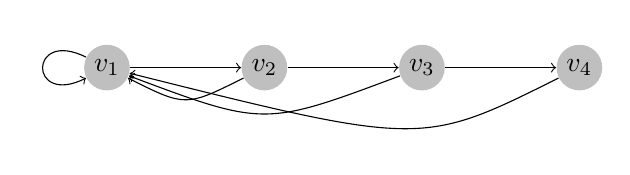
\begin{tikzpicture}[line join=bevel]
  \tikzstyle{vertex}=[circle,fill=black!25,minimum size=12pt,inner sep=2pt]
  \node[vertex] (G_1) at (-2,0) {$v_1$};
  \node[vertex] (G_2) at (0,0)  {$v_2$};
  \node[vertex] (G_3) at (2,0)   {$v_3$};
  \node[vertex] (G_4) at (4,0)   {$v_4$};
  \draw [->] (G_1) -- (G_2);
  \draw [->] (G_2) -- (G_3);
  \draw [->] (G_3) -- (G_4);
  \draw [->] (G_1) .. controls (-3.0, 0.5) and (-3.0, -0.5).. (G_1);
  \draw [->] (G_2) .. controls (-1.0, -0.5) .. (G_1);
  \draw [->] (G_3) .. controls (0.0, -0.75) .. (G_1);
  \draw [->] (G_4) .. controls (2.0, -1.0) .. (G_1);
\end{tikzpicture}
\caption{The graph used in proof of Theorem \ref{path-randomized-exponential} for $n=4$}
\label{graph-randomized}
\end{figure}

\section{Correctness for UPATH}\label{correctness-for-upath}

To show that our decider for UPATH based on RandomWalk really only
neeeds to do poly-bounded many steps, we are going to abstract from the
concrete algorithm and define a \emph{random walk on a graph}.

A \emph{random walk on a graph $G$ starting at $a$} is a \emph{infinite}
sequence of nodes $W = (v_1, v_2, \dots)$ where each $v_{i+1}$ was
choosen randomly under uniform distribution from the neighbour nodes of
$v_i$. (so $\{v_i, v_{i+1}\}$ is an egde in $G$)

We are now interested in the probability that a node $v$ occurs in this
sequence.

To do this, we are going to model the \emph{random walk on G} as a
\emph{Markov Chain}. We define the random variable $X_i$ as the node in
$G$ that is reached at the $i$-th step of our random walk. We can see
that, $X_i$ only depends on the value of $X_{i-1}$, the previous node,
so we know that:

\[ Pr[X_i = v | X_{i-1} = u] = \left\{
  \begin{array}{l l}
    \frac{1}{d(u)} & \quad \text{if $v$ is adjacent to $u$}\\
    0 & \quad \text{otherwise}
  \end{array} \right.
\]

Thus the sequence of random variables $X_1, X_2, X_3, ...$ has the
\emph{Markov Property}.

Furthermore we see that $Pr[X_i = v | X_{i-1} = u]$ only depends on $u$
and $v$ and not on $i$ from which we can conclude that this is a
\emph{stationary} markov chain.

This means it is rather easy to transform a graph into the state diagram
of a markov chain that models a random walk on this gaph: We replace the
undirected edges $\{u, v\}$ by directed edges $(u, v)$ and $(v, u)$ and
label them with the correct transition probabilities, $\frac{1}{d(u)}$
and $\frac{1}{d(v)}$ respectively. For an example see figure
\ref{graph-markov}.

Since each input graph is of finite size, we can define the
state-transition matrix $P \in \mathbb{R}^{n \times n}$

\begin{figure}
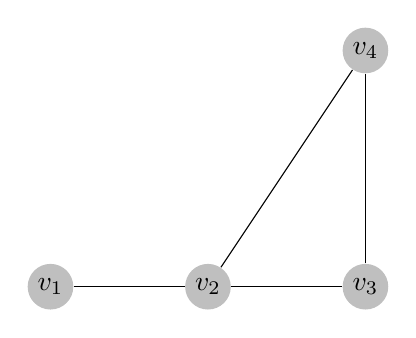
\begin{tikzpicture}[line join=bevel]
  \tikzstyle{vertex}=[circle,fill=black!25,minimum size=12pt,inner sep=2pt]
  \node[vertex] (G_1) at (-2,0)  {$v_1$};
  \node[vertex] (G_2) at (0,0)   {$v_2$};
  \node[vertex] (G_3) at (2,0)   {$v_3$};
  \node[vertex] (G_4) at (2,3)   {$v_4$};
  \draw (G_1) -- (G_2);
  \draw (G_2) -- (G_3);
  \draw (G_2) -- (G_4);
  \draw (G_3) -- (G_4);
\end{tikzpicture}
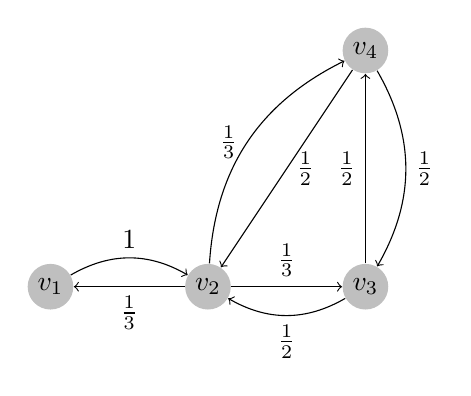
\begin{tikzpicture}[->,line join=bevel]
  \tikzstyle{vertex}=[circle,fill=black!25,minimum size=12pt,inner sep=2pt]
  \node[vertex] (G_1) at (-2,0)  {$v_1$};
  \node[vertex] (G_2) at (0,0)   {$v_2$};
  \node[vertex] (G_3) at (2,0)   {$v_3$};
  \node[vertex] (G_4) at (2,3)   {$v_4$};
  \path (G_1) edge [bend left] node[above] {1} (G_2)
        (G_2) edge node[below] {$\frac{1}{3}$} (G_1)
        (G_2) edge node[above] {$\frac{1}{3}$} (G_3)
        (G_3) edge [bend left] node[below] {$\frac{1}{2}$} (G_2)
        (G_2) edge [bend left] node[left] {$\frac{1}{3}$} (G_4)
        (G_4) edge node[right] {$\frac{1}{2}$} (G_2)
        (G_3) edge node[left] {$\frac{1}{2}$} (G_4)
        (G_4) edge [bend left] node[right] {$\frac{1}{2}$} (G_3);
\end{tikzpicture}
\caption{The original graph on the left, the state graph on the right.}
\label{graph-markov}
\end{figure}

\begin{enumerate}
\def\labelenumi{\arabic{enumi}.}
\item
  Show that
  $P_v = \lim{n \longrightarrow \infty} \frac{|\{i \leq n | v = v_i\}|}{n}$

  \begin{itemize}
  \itemsep1pt\parskip0pt\parsep0pt
  \item
    Proof that $P_{(u, v)} = \frac{1}{2 \cdot e}$
  \item
    Proof that $P_v = d(v) \cdot P_{(u, v)}$
  \end{itemize}
\item
  Show that the expected number of steps of a random walk of a to visit
  all nodes once is bounded by a polynominal.
\item
  Show that $b$ appears with probability higher than $\frac{1}{2}$ on
  such a random walk.
\end{enumerate}

\chapter{Universal Traversal
Sequence}\label{universal-traversal-sequence}

\section{Definition}\label{definition}

\begin{itemize}
\itemsep1pt\parskip0pt\parsep0pt
\item
  Visit all nodes in a d-regular Graph (why d-regular: formalism, node
  numbering..)
\end{itemize}

\section{Relation to previous proof}\label{relation-to-previous-proof}

\begin{itemize}
\itemsep1pt\parskip0pt\parsep0pt
\item
  usage of probability applicifcation (only finitly many d-regular
  graphs of a certain size)
\end{itemize}

% ~\citeNiklaus{DBLP:books/daglib/0094933}.
%\begin{figure}[!htb]
%  \centering
%  \includegraphics[width=10cm]{NAME/images/LaTeX-logo.png}
%  \caption{Lorem ipsum dolor sit amet, consetetur sadipscing elitr, sed diam.}
%  \label{fig:latex-logo}
%\end{figure} 

\bibliographystyleNiklaus{plain}
\bibliographyNiklaus{Niklaus/Literature}

